\documentclass[11pt]{article}

% --- Layout ---
\usepackage[margin=1in]{geometry}
\setlength{\parindent}{0pt}
\setlength{\parskip}{1\baselineskip}
\setlength{\emergencystretch}{2em}

% --- Math & Figures ---
\usepackage{amsmath, amssymb}
\usepackage{graphicx}
\usepackage{tikz}
\usetikzlibrary{decorations.pathreplacing}
\usepackage{fancyhdr}
\pagestyle{fancy}
\fancyhf{}
\fancyfoot[L]{\footnotesize Internal technical note}
\fancyfoot[R]{\footnotesize January 2026}
\renewcommand{\headrulewidth}{0pt}
\renewcommand{\footrulewidth}{0pt}

% --- Metadata ---
\title{Why the Arctic Breaks Temporal Systems First}
\author{}
\date{January 2026}

\begin{document}
\maketitle

\begin{abstract}
Long-horizon sensing systems fail in characteristic ways under extreme operational conditions. In the Arctic, intermittent connectivity, power constraints, environmental stress, and logistical latency expose a specific architectural weakness: time ceases to be reliably queryable. This note explains why temporal coherence degrades earliest in polar systems, how this failure manifests operationally, and why it is often misattributed to sensing or communications rather than system architecture.
\end{abstract}

% =========================
\section{Introduction}
% =========================

The Arctic is often treated as a special case in sensing and monitoring system design. Environmental extremes, sparse infrastructure, and limited access make deployment difficult and expensive. However, these same conditions make the Arctic a uniquely revealing environment for studying systemic failure modes.

In practice, Arctic systems do not fail because sensors stop working or data cannot be transmitted. Data continues to arrive. Dashboards continue to populate. What fails first is the ability to answer basic temporal questions: what happened when, what overlapped with what, and what could have been known at a given time.

This failure is subtle, cumulative, and often invisible until downstream trust is lost.

% =========================
\section{System Context}
% =========================

A typical Arctic sensing deployment involves some combination of:

\begin{itemize}
  \item Autonomous or semi-autonomous platforms (moorings, buoys, vehicles)
  \item Long-lived sensors operating without continuous GNSS
  \item Local buffering over days to months
  \item Intermittent uplink via satellite, aircraft, or seasonal retrieval
  \item Analysis performed far from the point of observation
\end{itemize}

Human operators are rarely co-located with the platform. Maintenance cycles are long. Connectivity windows are narrow and unpredictable. These constraints are not exceptional; they are the operating baseline.

% =========================
\section{Observed Failure Mode}
% =========================

The first failure observed in Arctic systems is temporal, not physical.

Sensor clocks drift over time. Buffered data is transmitted in bursts. Arrival time at the ingest system may lag the physical event by weeks. Despite this, timestamps are typically collapsed into a single scalar during ingestion, often privileging arrival time or applying undocumented correction heuristics.

The system remains operational, but its temporal model no longer corresponds cleanly to reality. Apparent correlations emerge that are artefacts of buffering and transport. Causal reasoning becomes unreliable, yet the degradation is rarely explicit.

Because data continues to flow, the failure is silent.

Figure 1 illustrates why this failure mode emerges earliest in polar systems: environmental and operational constraints accelerate the collapse of assumptions that normally keep time coherent.

% =========================
\section{Why the Arctic Exposes This First}
% =========================

The Arctic does not create the temporal problem; it removes the assumptions that normally hide it.

In temperate or well-connected environments, frequent synchronisation, human oversight, and short feedback loops mask temporal incoherence. Drift is corrected before it matters. Context is reconstructed informally.

In the Arctic, those stabilising factors are absent. Drift accumulates. Context is lost. Latency stretches. The same architectural assumptions now fail visibly and early.

What appears to be an Arctic-specific issue is, in fact, a general property revealed under stress.

% =========================
\section{Consequences}
% =========================

Once temporal coherence degrades, several downstream effects follow:

\begin{itemize}
  \item Alerts cannot be reliably attributed to causal precursors
  \item Cross-sensor correlations become suspect
  \item Post-hoc analysis cannot reconstruct what was known when
  \item Assurance and auditability are undermined
\end{itemize}

These failures are often misdiagnosed as data quality issues or communications limitations. In reality, they reflect an architectural gap in how time is represented and propagated.

% =========================
\section{Implications Beyond the Arctic}
% =========================

The Arctic is not unique. It is simply early.

Any system that is:
\begin{itemize}
  \item unmanned,
  \item long-horizon,
  \item intermittently connected, and
  \item expected to support autonomous or high-stakes decisions
\end{itemize}
will eventually encounter the same failure mode.

The Arctic serves as a proving ground not because it is exotic, but because it strips away assumptions that no longer hold as systems scale in autonomy and duration.

% =========================
\section{Conclusion}
% =========================

The Arctic breaks temporal systems first because it makes time visible. It exposes the limits of scalar timestamps, silent correction, and implicit assumptions about continuity.

Understanding this failure mode in polar systems provides an opportunity to address it architecturally—before it emerges elsewhere under less forgiving conditions.

\medskip

While the Arctic exposes this failure mode earliest, the underlying cause is not polar. It is architectural. Any system that operates without continuous synchronisation, human continuity, or low-latency feedback will eventually encounter the same loss of temporal coherence. The Arctic merely removes the assumptions that normally conceal it.

\emph{The architectural implications of this failure mode, and a minimal model for preserving temporal coherence under intermittency, are developed in a companion technical paper.}

\begin{figure}[ht]
\centering
\resizebox{\linewidth}{!}{
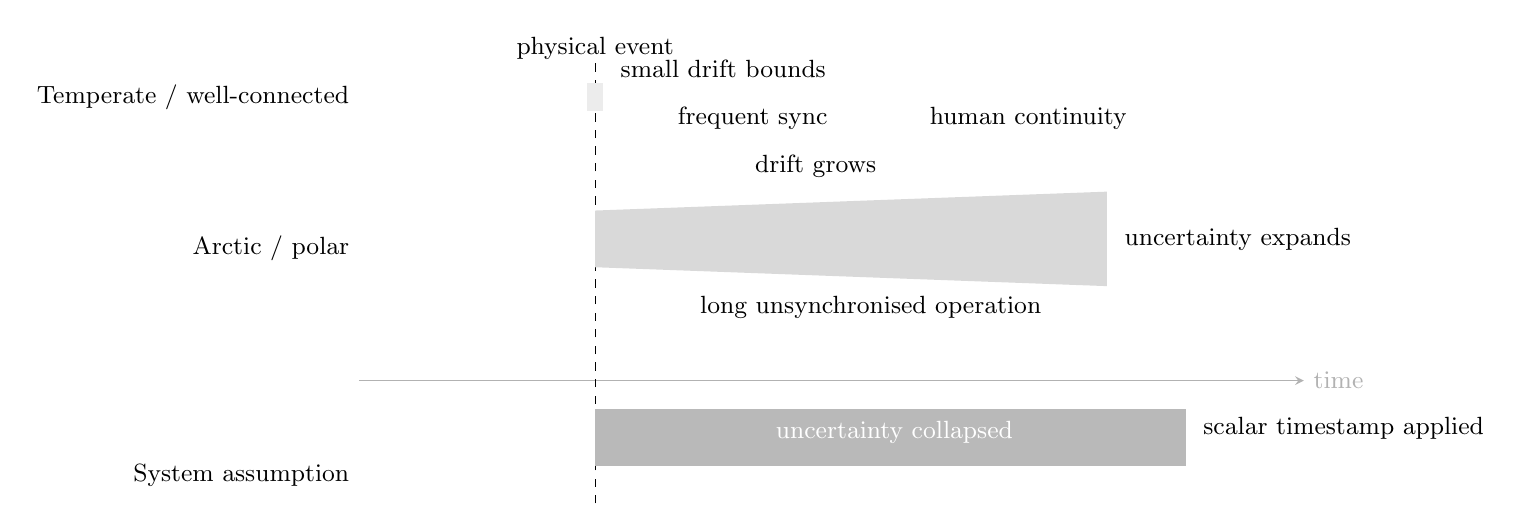
\begin{tikzpicture}[
  x=1cm,
  y=1.2cm, % <-- increases vertical spacing
  >=stealth,
  every node/.style={font=\small}
]

% Time axis
\draw[->, gray!60] (0,0) -- (12,0) node[right, gray!60]{time};

% Row labels (increased vertical separation)
\node[anchor=east] at (0,3.0) {Temperate / well-connected};
\node[anchor=east] at (0,1.4) {Arctic / polar};
\node[anchor=east] at (0,-1.0) {System assumption};

% Physical event reference
\draw[dashed] (3,-1.3) -- (3,3.4);
\node[above] at (3,3.3) {physical event};

% --- Row 1: Temperate ---
\fill[gray!15] (2.9,2.85) rectangle (3.1,3.15);
\node[above right] at (3.2,3.1) {small drift bounds};
\node[below] at (5,3) {frequent sync};
\node[below] at (8.5,3) {human continuity};

% --- Row 2: Arctic ---
\fill[gray!30] (3,1.2) -- (3,1.8) -- (9.5,2.0) -- (9.5,1.0) -- cycle;
\node[above] at (5.8,2.05) {drift grows};
\node[below] at (6.5,1.0) {long unsynchronised operation};
\node[right] at (9.6,1.5) {uncertainty expands};

% --- Row 3: System assumption ---
\fill[gray!55] (3,-0.9) rectangle (10.5,-0.3);
\node[white] at (6.8,-0.55) {uncertainty collapsed};
\node[right] at (10.6,-0.5) {scalar timestamp applied};

\end{tikzpicture}
}

\vspace{0.8em}

\centering
\emph{Time appears precise at exactly the point it becomes unreliable.}

\caption{
Why the Arctic breaks temporal systems first.
Frequent synchronisation and human continuity keep temporal uncertainty narrow in well-connected settings.
In polar deployments, drift accumulates and buffering dominates, expanding uncertainty over time.
Many systems nevertheless collapse this uncertainty into scalar timestamps at ingestion, creating apparent precision while causal ambiguity grows.
}
\end{figure}

\end{document}